\section{Campaign evaluation: what each stage was worth}\label{sec:eval}

The campaign ran from 2026-09-26 to 2026-09-29 on one Apple M5 Max workstation (18 cores), shared with unrelated jobs. It left 19 walk logs, four projection logs (the screen of the July certificates and three rounds) and a scoreboard that was re-scored after every batch, from which the following figures are computed by a script (\texttt{paper\_stats.py}, to be included in the release) that computes each number by two code paths or checks it against a known total.
A walk \emph{lowers} the rank if its result has smaller rank than its own seed; for projection children, whose seeds start unreduced, this is not a record.

\subsection{Volume}
In all, 4{,}816 walks were completed (a further 34 rows were rejected before any move because the seed file was stored in another orientation than the driver passed), totalling $3.103\times10^{11}$ proposals over 3{,}223 distinct seeds and 2{,}708 distinct formats: 3{,}530 walks of 40M proposals, 881 of 100M and 405 of 200M.
1{,}254 walks (26.0\%) lowered the rank, from 654 distinct seeds, removing 18{,}877 rank units in total, 15.05 per lowering walk on average (median 11, maximum 136); 97.5\% of the units come from projection children (S11 and S13 below).
Seed ranks ran from 21 to 12{,}769. CPU time was not logged; the per-limb rates of \cref{sec:walker} put the total at roughly 55 CPU-hours.

\subsection{Yield by seed class}
\Cref{tab:stages} groups the logs into stages by the origin of their seeds, and \cref{fig:yield} shows proposals per lowering walk on a logarithmic scale.
\begin{table}[t]
\centering\small
\begin{tabular}{@{}p{4.6cm}p{4.1cm}rrrr@{}}
\toprule
stage & seeds & walks & lowered & rate & moves/lowering\\
\midrule
S1 public integer schemes, 40M & best scheme per format, largest side 5--16 & 629 & 6 & 0.95\% & 4.2G\\
S2 same seeds, 200M restart & 281 of the above & 281 & 6 & 2.1\% & 9.4G\\
S3 continuation of S1 outputs, +200M & outputs that had lowered & 24 & 2 & 8.3\% & 2.4G\\
S4 alternative public schemes, 100M & 162 near-best schemes & 162 & 3 & 1.9\% & 5.4G\\
S5 fmm-schemes files, 100M & 17 & 34 & 11 & 32\% & 0.31G\\
S6 fmm-schemes release 1.1, 200M & 25 & 100 & 15 & 15\% & 1.3G\\
S7 matmulcatalog replays, pass 1, 40M & 263 & 526 & 39 & 7.4\% & 0.54G\\
S8 continuation of S7, +100M & outputs that had lowered & 80 & 22 & 27.5\% & 0.36G\\
S9 matmulcatalog replays, pass 2, 40M & 801 at or below a listed rank & 801 & 38 & 4.7\% & 0.84G\\
S10 closure products, 40M & 666 & 694 & 29 & 4.2\% & 0.96G\\
S11 projection children, 40M & 440 children & 880 & 792 & 90\% & 0.044G\\
S12 deepening, matmulcatalog lineage, 100M & 26 & 144 & 8 & 5.6\% & 1.8G\\
S13 deepening, projection lineage, 100M & 243 & 461 & 283 & 61\% & 0.16G\\
\midrule
all & 3{,}223 seeds & 4{,}816 & 1{,}254 & 26.0\% & 0.25G\\
\bottomrule
\end{tabular}
\caption{Walk yield by stage. ``Moves/lowering'' is total proposals divided by walks that lowered. Walks from replayed recipes and closure products lower by very little (median 1--2 terms, maximum 15 for closure products, 39 for replays); walks from projection children lower, when they lower, by a median of 16 terms (14.5 in the first pick of round 1).}
\label{tab:stages}
\end{table}

\begin{figure}[t]
\centering
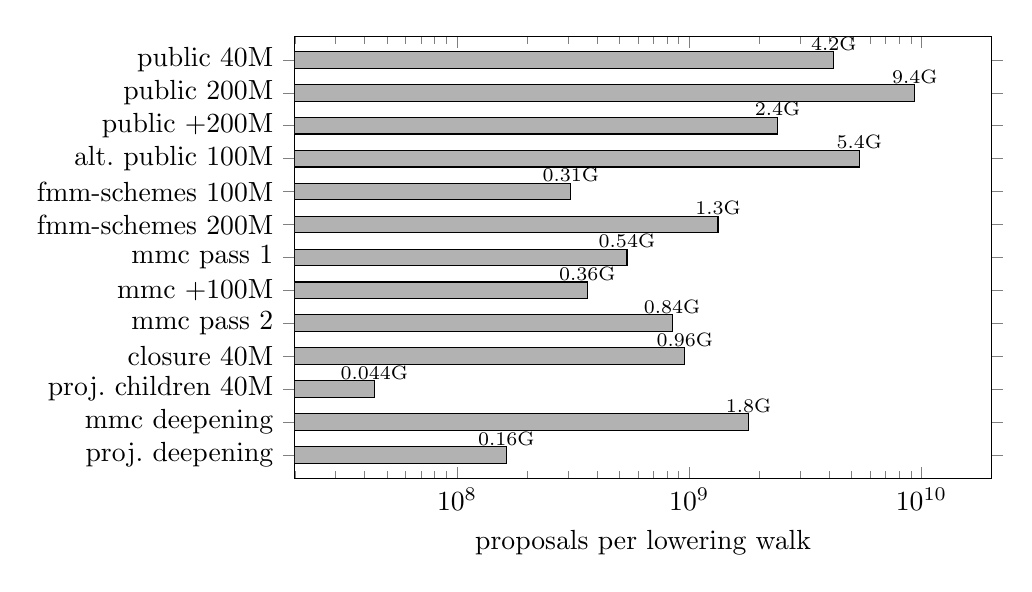
\begin{tikzpicture}
\begin{axis}[xbar,xmode=log,log origin=infty,width=0.86\textwidth,height=7.2cm,
  xmin=2e7,xmax=2e10,bar width=6pt,
  xlabel={proposals per lowering walk},
  symbolic y coords={S1,S2,S3,S4,S5,S6,S7,S8,S9,S10,S11,S12,S13},
  y dir=reverse,ytick=data,enlarge y limits=0.06,
  yticklabels={public 40M,public 200M,public +200M,alt.\ public 100M,fmm-schemes 100M,fmm-schemes 200M,mmc pass 1,mmc +100M,mmc pass 2,closure 40M,proj.\ children 40M,mmc deepening,proj.\ deepening},
  nodes near coords,every node near coord/.append style={font=\scriptsize},
  nodes near coords align={horizontal},
  point meta=explicit symbolic]
\addplot[fill=gray!60] coordinates {(4.19e9,S1) [4.2G] (9.37e9,S2) [9.4G] (2.4e9,S3) [2.4G] (5.4e9,S4) [5.4G] (3.09e8,S5) [0.31G] (1.33e9,S6) [1.3G] (5.39e8,S7) [0.54G] (3.64e8,S8) [0.36G] (8.43e8,S9) [0.84G] (9.57e8,S10) [0.96G] (4.4e7,S11) [0.044G] (1.8e9,S12) [1.8G] (1.63e8,S13) [0.16G]};
\end{axis}
\end{tikzpicture}
\caption{Proposals per lowering walk by stage (\cref{tab:stages}), logarithmic axis. Projection children are cheapest by one to two orders of magnitude, but their lowerings are relative to unreduced seeds.}
\label{fig:yield}
\end{figure}

Three regularities stand out. First, \emph{seeds that are already good rarely improve}: from 629 public integer schemes only six lowered at 40M proposals, every one of them at rank 486 or above; the 367 formats with a seed rank below 486 produced no lowering at all.
In the closure products, no walk from a seed of rank below 1{,}000 (291 walks) lowered, two of 433 below rank 2{,}000 did, against 27 of 261 above; 17 of the 29 lowerings occurred in the 68 walks whose format has a side equal to 11 (25\%, against 1.9\% elsewhere), for a reason we did not investigate.
Second, \emph{unreduced seeds improve almost always}, and this is most of the value of the projection stage for walking, on our reading: it produces seeds with slack.
Third, \emph{the pipeline finds its yield early and near the seed}: of the 228 records with a walk in their lineage (by the index's lineage labels, after correcting one label; walks that did not lower the rank are not counted, and counting them gives 229), the last walk was a 40M walk for 201, a 100M walk for 25 and a 200M walk for two. Most last walks were 40M walks, but 73\% of all walks were.

\subsection{Walk length and continuation}
Longer walks were tried in two ways. \emph{Restarts} walk the same seed again for longer with a different nonce. On the 281 public seeds a five-fold longer walk (200M against 40M) found exactly the six lowerings of the 40M screen and no other; across all 345 seeds walked at more than one length, longer walks produced three lowerings that shorter ones had missed (two from 40M to 100M, one from 100M to 200M), ended lower for 20 seeds, equal for 318 and \emph{higher} for seven.
\emph{Continuations} start from the output of an earlier walk that had lowered the rank, and these do pay: 22 of 80 continuation walks of replayed recipes lowered again (27.5\%), against 7.4\% for the fresh first pass, and 134 of 257 continuations of projection-child walks did (52\%).
Iterated deepening decays quickly: for the replayed-recipe lineage, the lowering rate by round was 8.3\%, 3.3\%, 0\%, 17\%, 0\%, 0\% over 60, 60, 12, 6, 3 and 3 walks.
The reading is that a walk finds what is nearby within the first tens of millions of proposals, and that a further walk from an \emph{improved} scheme has better odds than a longer walk from the same one; we did not test this against random restarts of matched cost.
One observation points the other way: a fresh 5M-proposal walk from the campaign's $24\times31\times32$ witness lowered it (\cref{tab:throughput}), so for that witness the 40M budget stopped short of stagnation; no other large format was tested.

\subsection{Cost of a record}
Dividing the proposals of each log by the records whose last walk came from it gives an upper bound on the price of a record (walks that produced nothing are included in the log's price): between 0.14G and 0.8G proposals for a record whose last walk was a 40M projection-child walk, between 0.45G (closure walks of round 2) and 10G (walks from the fmm-schemes release) for the other classes, and 1.4G on average over the 228 records with a walk if every proposal of the campaign is charged (1.0G if only the logs that ended a record are).
Records reached this way have small margins: for replay-then-walk chains the median margin below the best listed rank is 2 terms.
The large margins of the companion paper come from composition and from certificates produced by earlier stages, not from walks.

\subsection{Negative results}
In addition to those above: 162 alternative public schemes (same rank or one or two above the best) walked for 100M proposals gave three lowerings, each reaching the best public rank and none going below it; the second pass over replayed recipes lowered 38 of 801 at-rank seeds (4.7\%);
after the third round the rank-only closure has no lead left at or below the listed rank (one at 1\%), with the leaves of our scoreboard, which lacked the F2-only schemes of the literature that the companion paper's prior-art check used; and convergence of the projection cascade, which the campaign's notes claimed, is not established: its last pick was under-filled by the defect of \cref{sec:selfref}.
